\def\mytitle{BASIC OPTIMIZATION }
\def\myauthor{DUDEKULA USENI}
\def\contact{r171099@rguktrkv.ac.in}
\def\mymodule{Future Wireless Communication (FWC)}
\documentclass[10pt, a4paper]{article}
\usepackage[a4paper,outer=1.5cm,inner=1.5cm,top=1.75cm,bottom=1.5cm]{geometry}
\twocolumn
\usepackage{graphicx}
\graphicspath{{./images/}}
\usepackage[colorlinks,linkcolor={black},citecolor={blue!80!black},urlcolor={blue!80!black}]{hyperref}
\usepackage[parfill]{parskip}
\usepackage{lmodern}
\usepackage{tikz}
\usepackage{physics}
%\documentclass[tikz, border=2mm]{standalone}
%\usepackage{karnaugh-map}
%\documentclass{article}
\usepackage{tabularx}
%\usepackage{circuitikz}
\usepackage{enumitem}
\usetikzlibrary{calc}
\usepackage{amsmath}
\usepackage{amssymb}
\renewcommand*\familydefault{\sfdefault}
\usepackage{watermark}
\usepackage{lipsum}
\usepackage{xcolor}
\usepackage{listings}
\usepackage{float}
\usepackage{titlesec}
\providecommand{\mtx}[1]{\mathbf{#1}}
\titlespacing{\subsection}{1pt}{\parskip}{3pt}
\titlespacing{\subsubsection}{0pt}{\parskip}{-\parskip}
\titlespacing{\paragraph}{0pt}{\parskip}{\parskip}
\providecommand{\qfunc}[1]{\ensuremath{Q\left(#1\right)}}
\providecommand{\sbrak}[1]{\ensuremath{{}\left[#1\right]}}
\providecommand{\lsbrak}[1]{\ensuremath{{}\left[#1\right.}}
\providecommand{\rsbrak}[1]{\ensuremath{{}\left.#1\right]}}
\providecommand{\brak}[1]{\ensuremath{\left(#1\right)}}
\providecommand{\lbrak}[1]{\ensuremath{\left(#1\right.}}
\providecommand{\rbrak}[1]{\ensuremath{\left.#1\right)}}
\providecommand{\cbrak}[1]{\ensuremath{\left\{#1\right\}}}
\providecommand{\lcbrak}[1]{\ensuremath{\left\{#1\right.}}
\providecommand{\rcbrak}[1]{\ensuremath{\left.#1\right\}}}
\newcommand{\figuremacro}[5]{
    \begin{figure}[#1]
        \centering
        \includegraphics[width=#5\columnwidth]{#2}
        \caption[#3]{\textbf{#3}#4}
        \label{fig:#2}
    \end{figure}
}
\newcommand{\myvec}[1]{\ensuremath{\begin{pmatrix}#1\end{pmatrix}}}
\let\vec\mathbf
\lstset{
frame=single, 
breaklines=true,
columns=fullflexible
}
\thiswatermark{\centering \put(0,-110.0){
\includegraphics[scale=0.3]{logo.png}} }
\title{\mytitle}
\author{\myauthor\hspace{1em}\\\contact\\FWC22098\hspace{6.5em}IITH\hspace{0.5em}\mymodule\hspace{6em}Assignment-optimization}
\begin{document}
	\maketitle
	\tableofcontents
   \section{Problem}
If $\vec{p(x)}$ be a polynomial of degree 3 satisfying $\vec{p(\vec{-1})} = \vec{10}$, $\vec{p(1)} = \vec{-6}$ and $\vec{p(x)}$ has maximum at $\vec{x} = \vec{-1}$ and $\vec{p(x)}$ has minima at $\vec{x} = \vec{1}$. Find the distance between the local maximum and local minimum of the curve.
  \section{Solution}
Let the polynomial be\\
\begin{align}
p(x)=ax^3 + bx^2 + cx + d\\
p(-1) = -a + b – c + d = 10\\
p(1) = a + b + c + d = –6\\
 \frac{dp(-1)}{dx}= 3a – 2b + c = 0\\
\frac{dp'(1)}{dx}= 6a + 2b = 0
\end{align}
From equations (2), (3), (4), (5)\\
We have 4 equations and 4 unknowns\\
The general equation of a line is,\\
\begin{align}
\vec{n}^\top \vec{x} = \vec{c}\\
\vec{n} = \myvec{\vec{n_1}\hspace{2mm}\vec{n_2}\hspace{2mm}\vec{n_3}\hspace{2mm}\vec{n_4}\hspace{2mm}}
\end{align} 
where
\begin{align}
\vec{n_1}=\myvec{-1\\1\\-1\\1},\hspace{3mm} \vec{n_2}=\myvec{1\\1\\1\\1}, \hspace{3mm} \vec{n_3}=\myvec{3\\-2\\1\\0}, \hspace{3mm} \vec{n_4}=\myvec{6\\2\\0\\0}\\ 
\vec{c}=\myvec{10\\-6\\0\\0},\hspace{20mm}
\end{align} 
$$ 
\begin{bmatrix}
-1 & 1 & -1 & 1\\
 1 & 1 & 1 & 1\\
 3 &-2 & 1 & 0\\
 6 & 2 & 0 & 0\\
\end{bmatrix}^\top \vec{x} = \myvec{10\\-6\\0\\0}
$$
\begin{align}
\vec{x} = \vec{n^-}^\top \vec{c}
\end{align}
$$
\vec{x} = \begin{bmatrix}
0.0625 & -0.0625 & 0.125 & 0.125\\
-0.1875 & 0.1875 &-0.375 & 0.125\\
-0.5625 & 0.5625 & -0.125 & -0.125\\
 0.625 & 0.3125 & 0.375 & 0.125\\
\end{bmatrix}\myvec{10\\-6\\0\\0}
	$$
\begin{align}
\vec{x} = \myvec{1\\-3\\-9\\5}
\end{align}\\
So the values of a,b,c and d are 1,-3,-9 and 5 respectively.\\
Finally the cubic polynomial is\\ 
\begin{align}
p(x)=x^3 - 3x^2  - 9x + 5
\end{align}
 we can find the maxima of eq(12) by using gradient ascent method 
$\implies x_{n+1} = x_n + \alpha \nabla f(x_n) $\\
 \begin{align}
        \implies x_{n+1} &= x_n + \alpha \brak{3x^2 - 6x - 9}
    \end{align}
 Taking $x_0=0.5,\alpha=0.001$ and precision = 0.00000001, values obtained using python are:
    \begin{align}
        \boxed{\text{Maxima} = 9.999999999995849}\\
        \boxed{\text{Maxima Point} = -0.9999991682168597}
    \end{align}
 we can find the minima of eq(12) by using gradient descent method
 $\implies x_{n+1} = x_n - \alpha \nabla f(x_n) $\\
 \begin{align}
        \implies x_{n+1} &= x_n - \alpha \brak{3x^2 - 6x - 6}
    \end{align}
Taking $x_0=1.5,\alpha=0.001$ and precision = 0.00000001, values obtained using python are:
    \begin{align}
        \boxed{\text{Minima} = -21.999999999995847}\\
        \boxed{\text{Minima Point} = 2.999999168216859 }
    \end{align}
 The distance between the local maximum and local minimum of the curve\\
 \begin{align}
 A=(-0.9999991682168597 , 9.999999999995849)\\
 B=(2.999999168216859   ,-21.999999999995847)
 \end{align}
 \begin{align}
 ||A-B||=4\sqrt{65}
 \end{align}
 \section{Construction}
  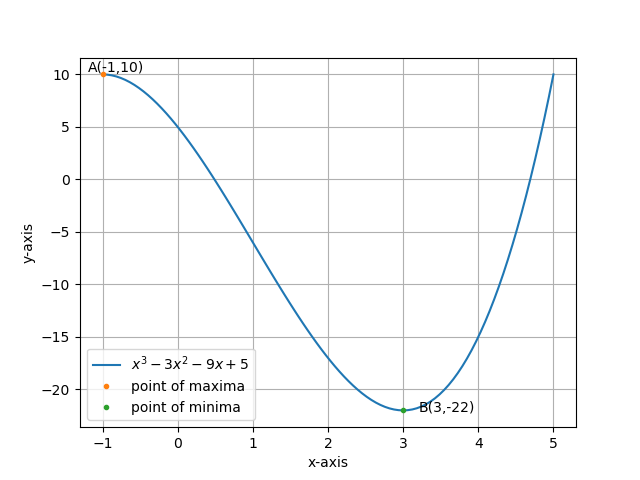
\includegraphics[scale=0.35]{op1.png}
  	\begin{center}
  Figure of construction
  	\end{center}
\section{Software}
\begin{center}
 \begin{lstlisting}
Below python code realizes the above construction :
https://github.com/dudekulauseni123/FWC0982022
 \end{lstlisting}
\end{center}
\end{document}
